\begin{dfn}[Plane Geometry]
Let \(P\) be an ordered geometry with a segment congruence and an angle congruence.
We say that \(P\) is a \emph{plane geometry} if the following properties are satisfied.
\begin{proplist}
\item \textbf{Right Angle Property.} Any two right angles are congruent.

\item \textbf{Circle-Ray Cut.} If \(o\), \(a\), and \(b\) are points such that \(a \neq o\) and \(b \neq o\), then there is a unique point \(c \in \RAY{o}{b}\) such that \(\SEGMENT{o}{c} \equiv \SEGMENT{o}{a}\).

\begin{center}
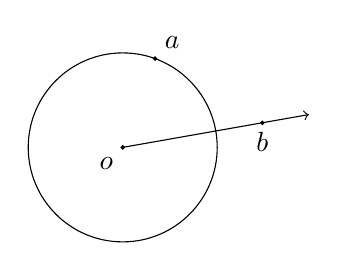
\begin{tikzpicture}[scale=0.6]
  \coordinate [label=below left:\(o\)]  (o) at (0  : 0);
  \draw [fill] (o) circle [radius=1pt];
  \coordinate [label=above right:\(a\)] (a) at (70 : 2);
  \draw [fill] (a) circle [radius=1pt];
  \coordinate [label=below:\(b\)]       (b) at (10 : 3);
  \draw [fill] (b) circle [radius=1pt];
  \draw [->] (o) -- (10: 4);
  \draw (o) circle [radius=2];
\end{tikzpicture}
\end{center}

\item \textbf{Circle-Circle Cut.} Let \(o\), \(a\), \(P\), and \(x\) be points, and suppose there are distinct points \(u\) and \(v\) on \(\CIRCLE{p}{x}\) such that \(u \in \INTCIRCLE{o}{a}\) and \(v \in \EXTCIRCLE{o}{a}\). Then \(\CIRCLE{o}{a} \cap \CIRCLE{p}{x}\) contains two distinct points.

\begin{center}
\begin{tikzpicture}[scale=0.6]
  \coordinate [label=below left:{\(o\)}]  (o) at (0,0);
  \draw [fill] (o) circle [radius=1pt];
  \coordinate [label=above left:{\(a\)}] (a) at ($ (o)+(140 : 2) $);
  \draw [fill] (a) circle [radius=1pt];
  \draw (o) circle [radius=2];

  \coordinate [label=below left:\(p\)]  (p) at (4,0);
  \draw [fill] (p) circle [radius=1pt];
  \coordinate [label=below right:\(x\)] (x) at ($ (p)+(320 : 3) $);
  \draw [fill] (x) circle [radius=1pt];
  \coordinate [label=below right:\(u\)] (u) at ($ (p)+(170 : 3) $);
  \draw [fill] (u) circle [radius=1pt];
  \coordinate [label=below right:\(v\)] (v) at ($ (p)+(20  : 3) $);
  \draw [fill] (v) circle [radius=1pt];
  \draw (p) circle [radius=3];
\end{tikzpicture}
\end{center}

\item \textbf{Circle Cut Transfer.} Suppose \(a\), \(b\), \(c\), \(d\), \(x\), \(y\), \(z\), and \(w\) are points such that \(\SEGMENT{a}{b} \equiv \SEGMENT{x}{y}\), \(\SEGMENT{b}{c} \equiv \SEGMENT{y}{z}\), and \(\SEGMENT{c}{d} \equiv \SEGMENT{z}{w}\). If \(\CIRCLE{b}{a} \cap \CIRCLE{c}{d}\) is not empty, then \(\CIRCLE{y}{x} \cap \CIRCLE{z}{w}\) is not empty.

\item \textbf{Angle-Side Congruence.} Suppose \(a\), \(b\), \(c\), \(x\), \(y\), and \(z\) are points such that \(\SEGMENT{b}{a} \equiv \SEGMENT{y}{x}\) and \(\SEGMENT{b}{c} \equiv \SEGMENT{y}{z}\). Then \(\SEGMENT{a}{c} \equiv \SEGMENT{x}{z}\) if and only if \(\ANGLE{a}{b}{c} \equiv \ANGLE{x}{y}{z}\).
\end{proplist}
\end{dfn}

The Circle Separation and Circle Cut properties allow us to construct points on the intersection of a circle with a central ray and of two circles, respectively. (Without these we have no way to construct points on circles!) The Circle Cut Transfer property says that our geometry is ``uniform'' in some sense, allowing us to shift points in the intersection of two circles. Angle-Side Congruence provides an essential link between segment congruence and angle congruence, which are otherwise unrelated.

\subsection*{Some Consequences}

In the remainder of this section, suppose \(P\) is a plane geometry.

\begin{prop}[Circle Trichotomy]
Let \(o\) and \(a\) be distinct points. Then \(\CIRCLE{o}{a}\), \(\INTCIRCLE{o}{a}\), and \(\EXTCIRCLE{o}{a}\) partition the set of points in \(P\). That is, every point is either on \(\CIRCLE{o}{a}\), interior to \(\CIRCLE{o}{a}\), or exterior to \(\CIRCLE{o}{a}\).
\end{prop}

\begin{prop}[SSS Theorem]
If two triangles can be labeled such that corresponding sides are congruent, then the triangles are congruent. More precisely, let \(a\), \(b\), and \(c\) be distinct points and \(x\), \(y\), and \(z\) be distinct points. If \(\SEGMENT{a}{b} \equiv \SEGMENT{x}{y}\), \(\SEGMENT{b}{c} \equiv \SEGMENT{y}{z}\), and \(\SEGMENT{c}{a} \equiv \SEGMENT{z}{x}\), then \(\TRIANGLE{a}{b}{c} \equiv \TRIANGLE{x}{y}{z}\).
\end{prop}

\begin{proof}
That \(\ANGLE{a}{b}{c} \equiv \ANGLE{x}{y}{z}\), \(\ANGLE{b}{c}{a} \equiv \ANGLE{y}{z}{x}\), and \(\ANGLE{z}{x}{y} \equiv \ANGLE{c}{a}{b}\) follows from three applications of the Angle-Side Congruence property.
\end{proof}

\begin{prop}[Uniqueness of Circle Cuts]
Let \(o\), \(a\), \(P\), \(x\), and \(h\) be points, with \(o\) and \(P\) distinct and with \(h\) not on \(\LINE{o}{p}\). There is at most one point \(u \in \CIRCLE{o}{a} \cap \CIRCLE{p}{x}\) on the \(h\)-side of \(\LINE{o}{p}\).
\end{prop}

\begin{proof}
Suppose we have two such points, \(u\) and \(v\). That is, both \(u\) and \(v\) are on the \(h\)-side of \(\LINE{o}{p}\) and \(u,v \in \CIRCLE{o}{a} \cap \CIRCLE{p}{x}\). Note that \(\SEGMENT{o}{p} \equiv \SEGMENT{o}{p}\), \(\SEGMENT{p}{u} \equiv \SEGMENT{p}{x} \equiv \SEGMENT{p}{v}\), and \(\SEGMENT{u}{o} \equiv \SEGMENT{a}{o} \equiv \SEGMENT{v}{o}\). By the SSS Theorem, we have \(\TRIANGLE{u}{o}{p} \equiv \TRIANGLE{v}{o}{p}\). In particular, we have \(\ANGLE{u}{o}{p} \equiv \ANGLE{v}{o}{p}\) and \(\ANGLE{u}{p}{o} \equiv \ANGLE{v}{p}{o}\). Now by AC7, we have \(v \in \RAY{o}{u} \subseteq \LINE{o}{u}\) and \(u \in \RAY{p}{v} \subseteq \LINE{p}{v}\). That is, \(u\) and \(v\) are points in the intersection of the lines \(\LINE{o}{u}\) and \(\LINE{p}{v}\). Since \(o\) and \(P\) are distinct, these lines must be distinct, and so they intersect at a unique point. Hence \(u = v\).
\end{proof}

\begin{prop}[SAS Theorem]
If two triangles can be labeled such that two corresponding sides, and the angles between, are congruent, then the triangles are congruent. More precisely, let \(a\), \(b\), and \(c\) be distinct points, and \(x\), \(y\), and \(z\) be distinct points. If \(\SEGMENT{a}{b} \equiv \SEGMENT{x}{y}\), \(\SEGMENT{b}{c} \equiv \SEGMENT{y}{z}\), and \(\ANGLE{a}{b}{c} \equiv \ANGLE{x}{y}{z}\), then \(\TRIANGLE{a}{b}{c} \equiv \TRIANGLE{x}{y}{z}\).
\end{prop}

\begin{prop}[Pons Asinorum (Bridge of Asses)]
If \(\TRIANGLE{a}{b}{c}\) is isoceles with \(\SEGMENT{a}{b} \equiv \SEGMENT{b}{c}\), then \(\ANGLE{b}{a}{c} \equiv \ANGLE{b}{c}{a}\).
\end{prop}

\begin{proof}
We have two triangles, \(\TRIANGLE{b}{a}{c}\) and \(\TRIANGLE{b}{c}{a}\), such that \(\SEGMENT{b}{c}\equiv \SEGMENT{b}{a}\), \(\SEGMENT{b}{a} \equiv \SEGMENT{b}{c}\), and \(\ANGLE{c}{b}{a} \equiv \SEGMENT{a}{b}{c}\). By the SAS Theorem, \(\TRIANGLE{b}{a}{c} \equiv \SEGMENT{b}{c}{a}\), and thus \(\ANGLE{b}{a}{c} \equiv \ANGLE{b}{c}{a}\).
\end{proof}

\begin{cor}
Every triangle which is equilateral is also equiangular; all three interior angles are congruent.
\end{cor}

\begin{construct}[equilateral triangle with a given side]
Given distinct points \(x\) and \(y\), there exist points \(z_1\) and \(z_2\), on opposite sides of \(\LINE{x}{y}\), such that \(\TRIANGLE{x}{y}{z_1}\) and \(\TRIANGLE{x}{y}{z_2}\) are equilateral. In fact, we have \(\TRIANGLE{x}{y}{z_1} \equiv \TRIANGLE{x}{y}{z_2}\).
\end{construct}

\begin{proof}
Consider the line \(\LINE{x}{y}\). By the Interpolation property, there exists a point \(u\) such that \(\BETWEEN{u}{x}{y}\). By the Circle Separation property, there is a point \(w \in \CIRCLE{y}{x} \cap \RAY{x}{w}\). Note in particular that \(\BETWEEN{w}{x}{y}\), and hence \(w\) is exterior to the circle \(\CIRCLE{y}{x}\). Moreover, \(w\) is on \(\CIRCLE{x}{y}\). Now \(y\) is also on \(\CIRCLE{x}{y}\), and by definition, \(y\) is interior to \(\CIRCLE{y}{x}\). By the Circle Cut property, there exist two points in \(\CIRCLE{x}{y} \cap \CIRCLE{y}{x}\), say \(z_1\) and \(z_2\), which must be on opposite sides of \(\LINE{x}{y}\) by the uniqueness of circle cuts. Now \(\SEGMENT{x}{z_1} \equiv \SEGMENT{x}{y} \equiv \SEGMENT{y}{z_1}\) and \(\SEGMENT{x}{z_2} \equiv \SEGMENT{x}{y} \equiv \SEGMENT{y}{z_2}\) by the definition of circles, so that \(\TRIANGLE{x}{y}{z_1}\) and \(\TRIANGLE{x}{y}{z_2}\) are equilateral by definition. Moreover, \(\TRIANGLE{x}{y}{z_1} \equiv \TRIANGLE{x}{y}{z_2}\) by the transitivity of segment congruence and the SSS Theorem.
\end{proof}

\begin{prop}[Segment Addition Theorem]
Suppose \(\BETWEEN{a}{b}{c}\) and \(\BETWEEN{x}{y}{z}\). If any two of \(\SEGMENT{a}{b} \equiv \SEGMENT{x}{y}\), \(\SEGMENT{b}{c} \equiv \SEGMENT{y}{z}\), and \(\SEGMENT{a}{c} \equiv \SEGMENT{x}{z}\) hold, then so does the third.
\end{prop}

\begin{proof}
Note that \(\ANGLE{a}{b}{c} \equiv \ANGLE{x}{y}{z}\), \(\ANGLE{b}{c}{a} \equiv \ANGLE{y}{z}{x}\), and \(\ANGLE{c}{a}{b} \equiv \ANGLE{z}{x}{y}\) by AC4. The result then follows from the SAS Theorem.
\end{proof}

\begin{lem}
Suppose \(\BETWEEN{a}{b}{c}\) and \(y \in \RAY{x}{z}\). If \(\SEGMENT{a}{b} \equiv \SEGMENT{x}{y}\) and \(\SEGMENT{a}{c} \equiv \SEGMENT{x}{z}\), then \(\BETWEEN{x}{y}{z}\).
\end{lem}

\begin{proof}
Since \(y \in \RAY{x}{z}\), we have four possibilities: \(y = x\), \(\BETWEEN{x}{y}{z}\), \(y = z\), and \(\BETWEEN{x}{z}{y}\). If \(y = x\), then we have \(\SEGMENT{a}{b} \equiv \SEGMENT{x}{x}\), so that \(b = a\), a contradiction. Similarly if \(y = z\) then we have \(\SEGMENT{x}{y} \equiv \SEGMENT{x}{z}\), so that \(y = z\), also a contradiction. Now suppose that \(\BETWEEN{x}{z}{y}\). Note that \(\ANGLE{c}{a}{b} \equiv \ANGLE{z}{x}{y}\), \(\SEGMENT{a}{c} \equiv \SEGMENT{x}{z}\), and \(\SEGMENT{a}{b} \equiv \SEGMENT{x}{y}\); by the SAS Theorem, \(\TRIANGLE{a}{b}{c} \equiv \TRIANGLE{x}{y}{z}\). In particular, the flat angle \(\ANGLE{a}{c}{b}\) is congruent to the straight angle \(\ANGLE{x}{z}{y}\), a contradiction. Thus \(\BETWEEN{x}{y}{z}\) as claimed.
\end{proof}

\begin{construct}[copy a segment onto a ray]
Let \(a\) and \(b\) be distinct points, and let \(o\) and \(t\) be distinct points.
There exists a point \(x\) on \(\RAY{o}{t}\) such that \(\SEGMENT{o}{x} \equiv \SEGMENT{a}{b}\).
\end{construct}

\begin{proof}
First we construct a point \(z\) such that \(\TRIANGLE{a}{o}{z}\) is equilateral; now \(\SEGMENT{z}{a} \equiv \SEGMENT{z}{o}\).
Using the Interpolation property, construct a point \(h\) such that \(\BETWEEN{z}{a}{h}\), and using the Circle Separation property, construct a point \(u\) on \(\RAY{a}{h}\) such that \(\SEGMENT{a}{u} \equiv \SEGMENT{a}{b}\).
Again using Circle Separation, construct a point \(v\) on \(\RAY{z}{o}\) such that \(\SEGMENT{z}{v} \equiv \SEGMENT{z}{u}\).
By the previous proposition, \(\BETWEEN{z}{o}{v}\).
Now \(\SEGMENT{z}{a} \equiv \SEGMENT{z}{o}\) and \(\SEGMENT{z}{u} \equiv \SEGMENT{z}{v}\), thus \(\SEGMENT{a}{u} \equiv \SEGMENT{o}{v}\). Again using Circle Separation, construct a point \(x\) on \(\RAY{o}{t}\) such that \(\SEGMENT{o}{x} \equiv \SEGMENT{o}{v}\). Then we have \(\SEGMENT{o}{x} \equiv \SEGMENT{o}{v} \equiv \SEGMENT{a}{u} \equiv \SEGMENT{a}{b}\) as needed.
\end{proof}

\begin{construct}[copy an angle onto a ray]
Let \(a\), \(o\), \(b\) be distinct noncollinear points and let \(P\) and \(x\) be distinct points. There exist two points \(y_1\) and \(y_2\), on opposite sides of \(\LINE{p}{x}\), such that \(\ANGLE{x}{p}{y_1} \equiv \ANGLE{x}{p}{y_2} \equiv \ANGLE{a}{o}{b}\). 
\end{construct}

\begin{proof}
First copy segment \(\SEGMENT{o}{b}\) onto \(\RAY{p}{x}\) at the point \(u\), then copy the segment \(\SEGMENT{b}{a}\) onto the ray \(\RAY{u}{p}\) at the point \(v\). Now copy \(\SEGMENT{o}{a}\) onto \(\RAY{p}{x}\) at the point \(w\). Note that \(\SEGMENT{o}{a} \equiv \SEGMENT{p}{w}\), \(\SEGMENT{o}{b} \equiv \SEGMENT{p}{u}\), and \(\SEGMENT{b}{a} \equiv \SEGMENT{u}{v}\). Moreover, the intersection \(\CIRCLE{o}{a} \cap \CIRCLE{b}{a}\) is nonempty, as it contains \(a\). By the Circle Cut Transfer property, \(\CIRCLE{p}{w} \cap \CIRCLE{u}{v}\) contains two points \(z_1\) and \(z_2\) on opposite sides of \(\LINE{p}{x}\). By the SSS Theorem, we have \(\TRIANGLE{p}{u}{z_1} \equiv \TRIANGLE{o}{b}{a} \equiv \TRIANGLE{p}{u}{z_2}\), and thus \(\ANGLE{u}{p}{z_1} \equiv \ANGLE{a}{o}{b} \equiv \ANGLE{u}{p}{z_2}\) as needed.
\end{proof}

\begin{prop}[ASA Theorem]
Let \(a\), \(b\), \(c\) be distinct noncollinear points, and let \(x\), \(y\), \(z\) be distinct points. If \(\ANGLE{a}{b}{c} \equiv \ANGLE{x}{y}{z}\), \(\SEGMENT{b}{c} \equiv \SEGMENT{y}{z}\), and \(\ANGLE{b}{c}{a} \equiv \ANGLE{y}{z}{x}\), then \(\TRIANGLE{a}{b}{c} \equiv \TRIANGLE{x}{y}{z}\).
\end{prop}

\begin{proof}
Copy \(\SEGMENT{y}{x}\) onto \(\RAY{b}{a}\) at \(d\).
Note that \(d\) and \(a\) are on the same side of \(\LINE{b}{c}\).
Moreover, we have \(\TRIANGLE{d}{b}{c} \equiv \TRIANGLE{x}{y}{z}\) by the SAS Theorem, and so \(\ANGLE{b}{c}{d} \equiv \ANGLE{y}{z}{x} \equiv \ANGLE{b}{c}{a}\).
By AC7, we have \(d \in \RAY{c}{a}\).
Now \(d\) is on both \(\LINE{b}{a}\) and \(\LINE{c}{a}\), and since \(a\), \(b\), and \(c\) are not collinear, we must have \(d = a\).
So \(\TRIANGLE{a}{b}{c} \equiv \TRIANGLE{x}{y}{z}\) as claimed.
\end{proof}

\begin{prop}[Angle Addition Theorem]
Suppose \(B \in \INTANGLE{A}{O}{C}\) and \(Y \in \INTANGLE{X}{P}{Z}\).
If any two of \(\ANGLE{A}{O}{C} \equiv \ANGLE{X}{P}{Z}\), \(\ANGLE{A}{O}{B} \equiv \ANGLE{X}{P}{Y}\), and \(\ANGLE{B}{O}{C} \equiv \ANGLE{Y}{P}{Z}\) holds, then so does the third.
\end{prop}

\begin{proof}
(write this. Uses SAS and segment addition.)
\end{proof}
